\section{Arquitectura}

En esta secci�n presentaremos y analizaremos la arquitectura pensada para resolver el trabajo, as� como las t�cticas utilizadas para asegurar los atributos de calidad que se mencionaron anteriormente.

\subsection{Comunicaci�n con Drones}

Para el monitoreo de las plantaciones se utilizar�n drones que tomar�n fotograf�as y luego ser�n analizadas para recaudar la informaci�n necesaria.  Para esto, contamos con un componente dedicado a la comunicaci�n con las interfaces de manejo de drones que nos provee el Ministerio y la empresa privada. Se utilizar� por default el sistema de drones estatales, en caso de no responder a los pedidos, se pasara a utilizar el sistema privado.





\begin{figure}[h!]
  \centering
  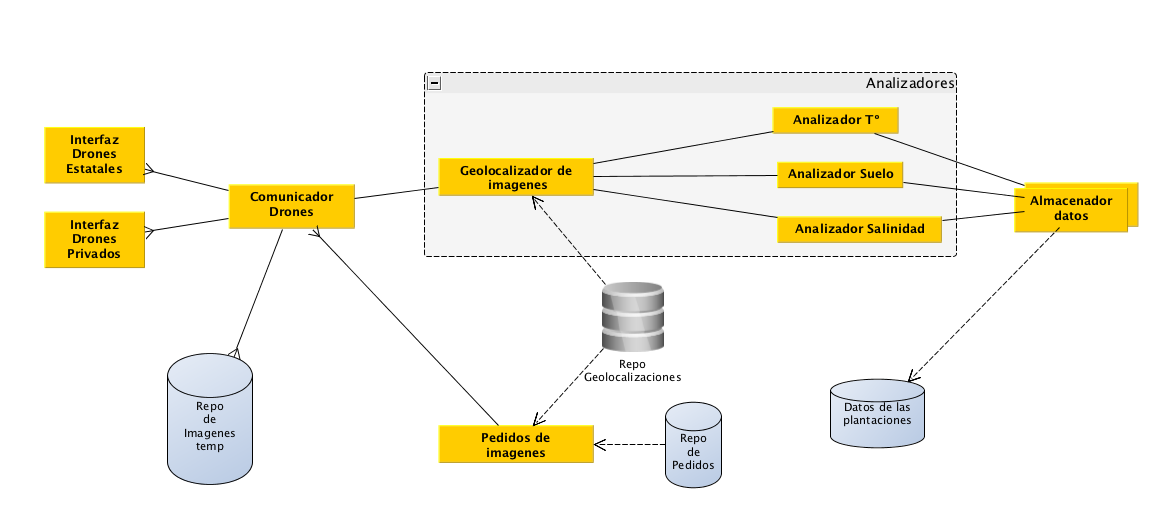
\includegraphics[width=1\textwidth]{./images/arq_drones.png}
  \caption{Arquitectura de comunicaci\'on con drones y procesamiento de im\'agenes}
  \label{fig:clases4}
\end{figure}

\begin{figure}[h!]
  \centering
  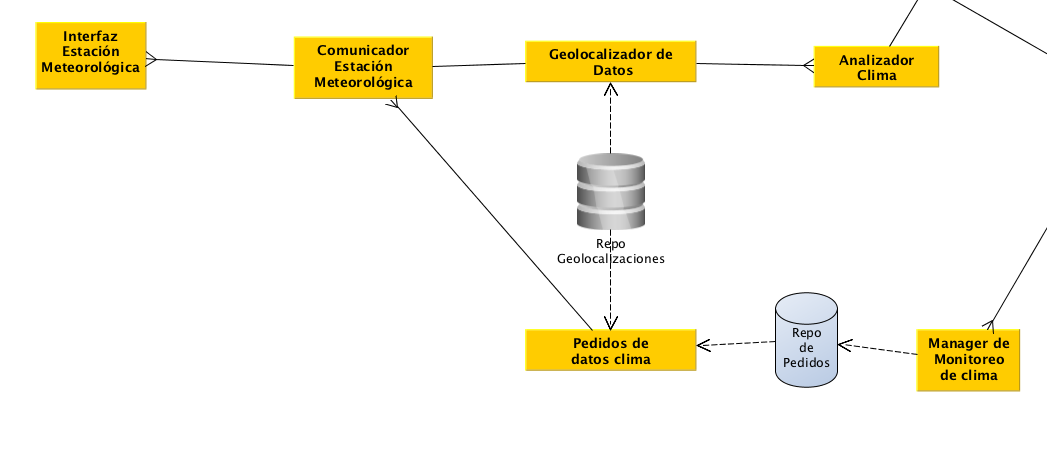
\includegraphics[width=1\textwidth]{./images/arq_clima.png}
  \caption{Arquitectura de comunicaci\'on con estaciones meteorol\'ogicas y procesamiento de datos}
  \label{fig:clases4}
\end{figure}

\begin{figure}[h!]
  \centering
  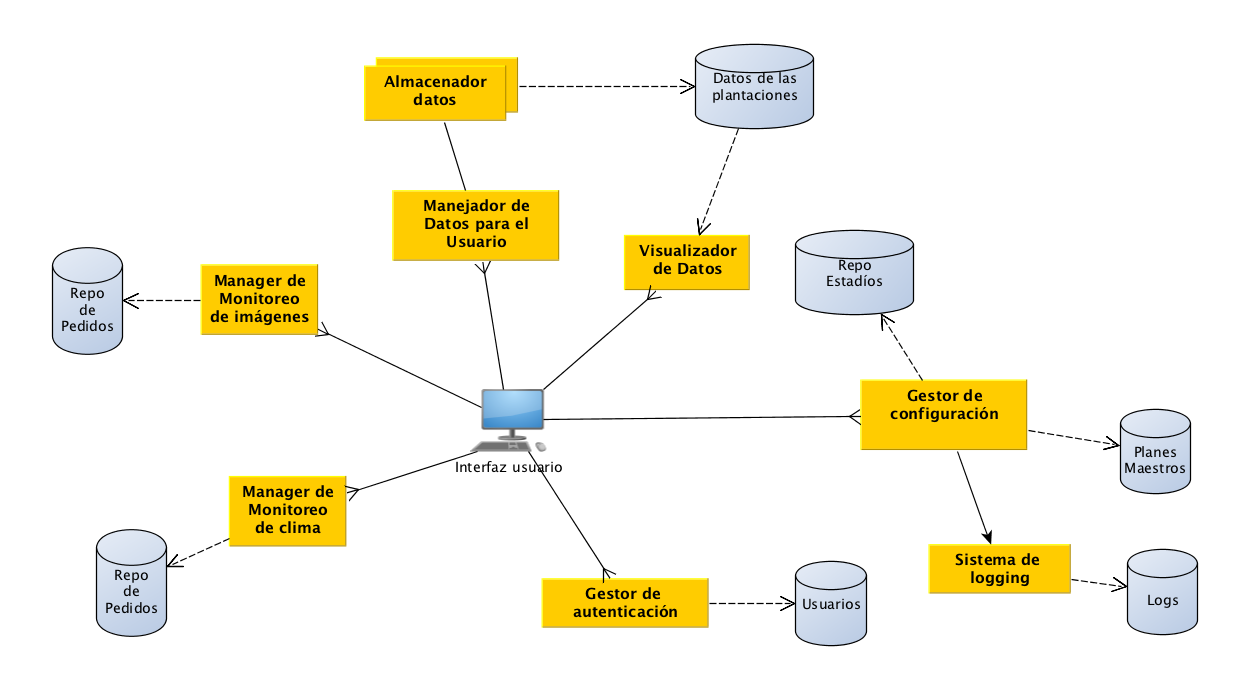
\includegraphics[width=0.4\textwidth]{./images/arq_interfazusuario.png}
  \caption{Arquitectura de comunicaci\'on con la interfaz de usuario}
  \label{fig:clases4}
\end{figure}

\begin{figure}[h!]
  \centering
  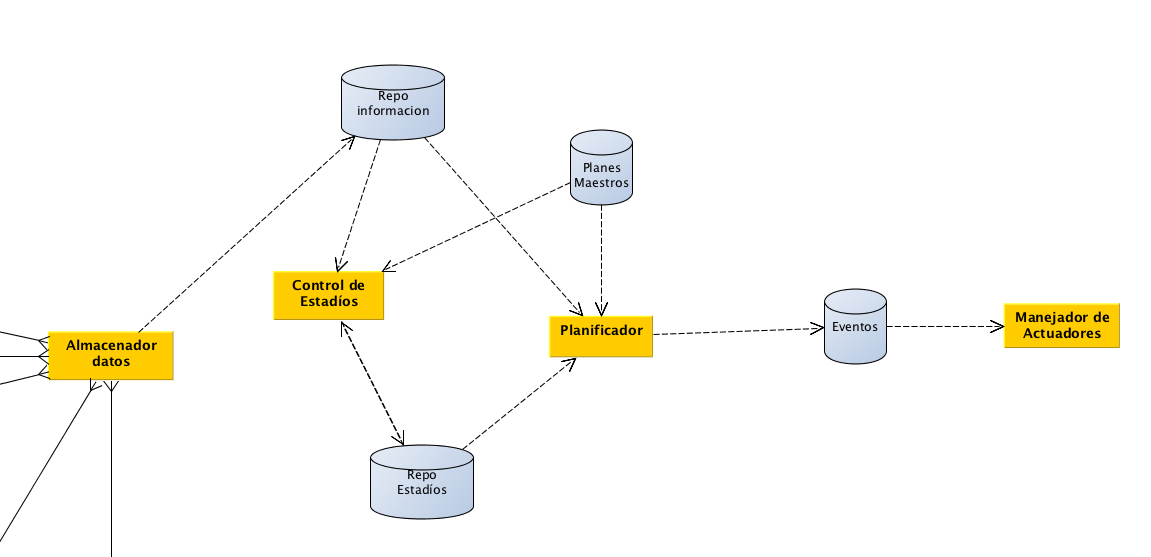
\includegraphics[width=1\textwidth]{./images/arq_plan.png}
  \caption{Arquitectura de planificaci\'on de eventos}
  \label{fig:clases4}
\end{figure}